\subsection{Project Binder}\label{seq:project-binder}

The Binder Project \cite{binder} (\url{https://jupyter.org/binder}) is
a sub project of the Jupyter project. The Binder project is formally operating
within the Jupyter ecosystem, but not confined to be useful only for notebooks.

The key components of the Binder software are \repotodocker{}
(Section~\ref{sec:repo2docker}) and \binderhub{}. The \repotodocker{} tool
creates a software environment inside a Docker container from a software
specification in a repository. \binderhub{} starts a Jupyter notebook server
within this container from which the user can execute the notebooks from the
repository.

\emph{\mybinder{}} (see \ref{sec:mybinder}) is a service provided by the \emph{BinderHub
Federation} that collectively host a service running the Binder software
under the URL \url{https://mybinder.org}. This is the service we made use of in
our example in section~\ref{sec:reproducibility-example}. The \emph{BinderHub Federation}

The focus for this proposal is to improve \repotodocker{}. In particular,
\repotodocker{} solves the software environment challenge (see
Section~\ref{sec:reproducibility-concept}) in a generic way and is independent
from Jupyter notebooks.

\TODO{Add image that depicts this Jupyter/Binder relation ship}.

\subsubsection{Basic functionality of Binder}
\label{binder-how-does-it-work}

The currently most common reproducibility use case -- with the current state of the Binder
tools -- is the one we introduced in
Section~\ref{sec:reproducibility-example}. We will use this to
describe the role of the individual components of Binder:


\begin{figure}[ht]
  \centering
    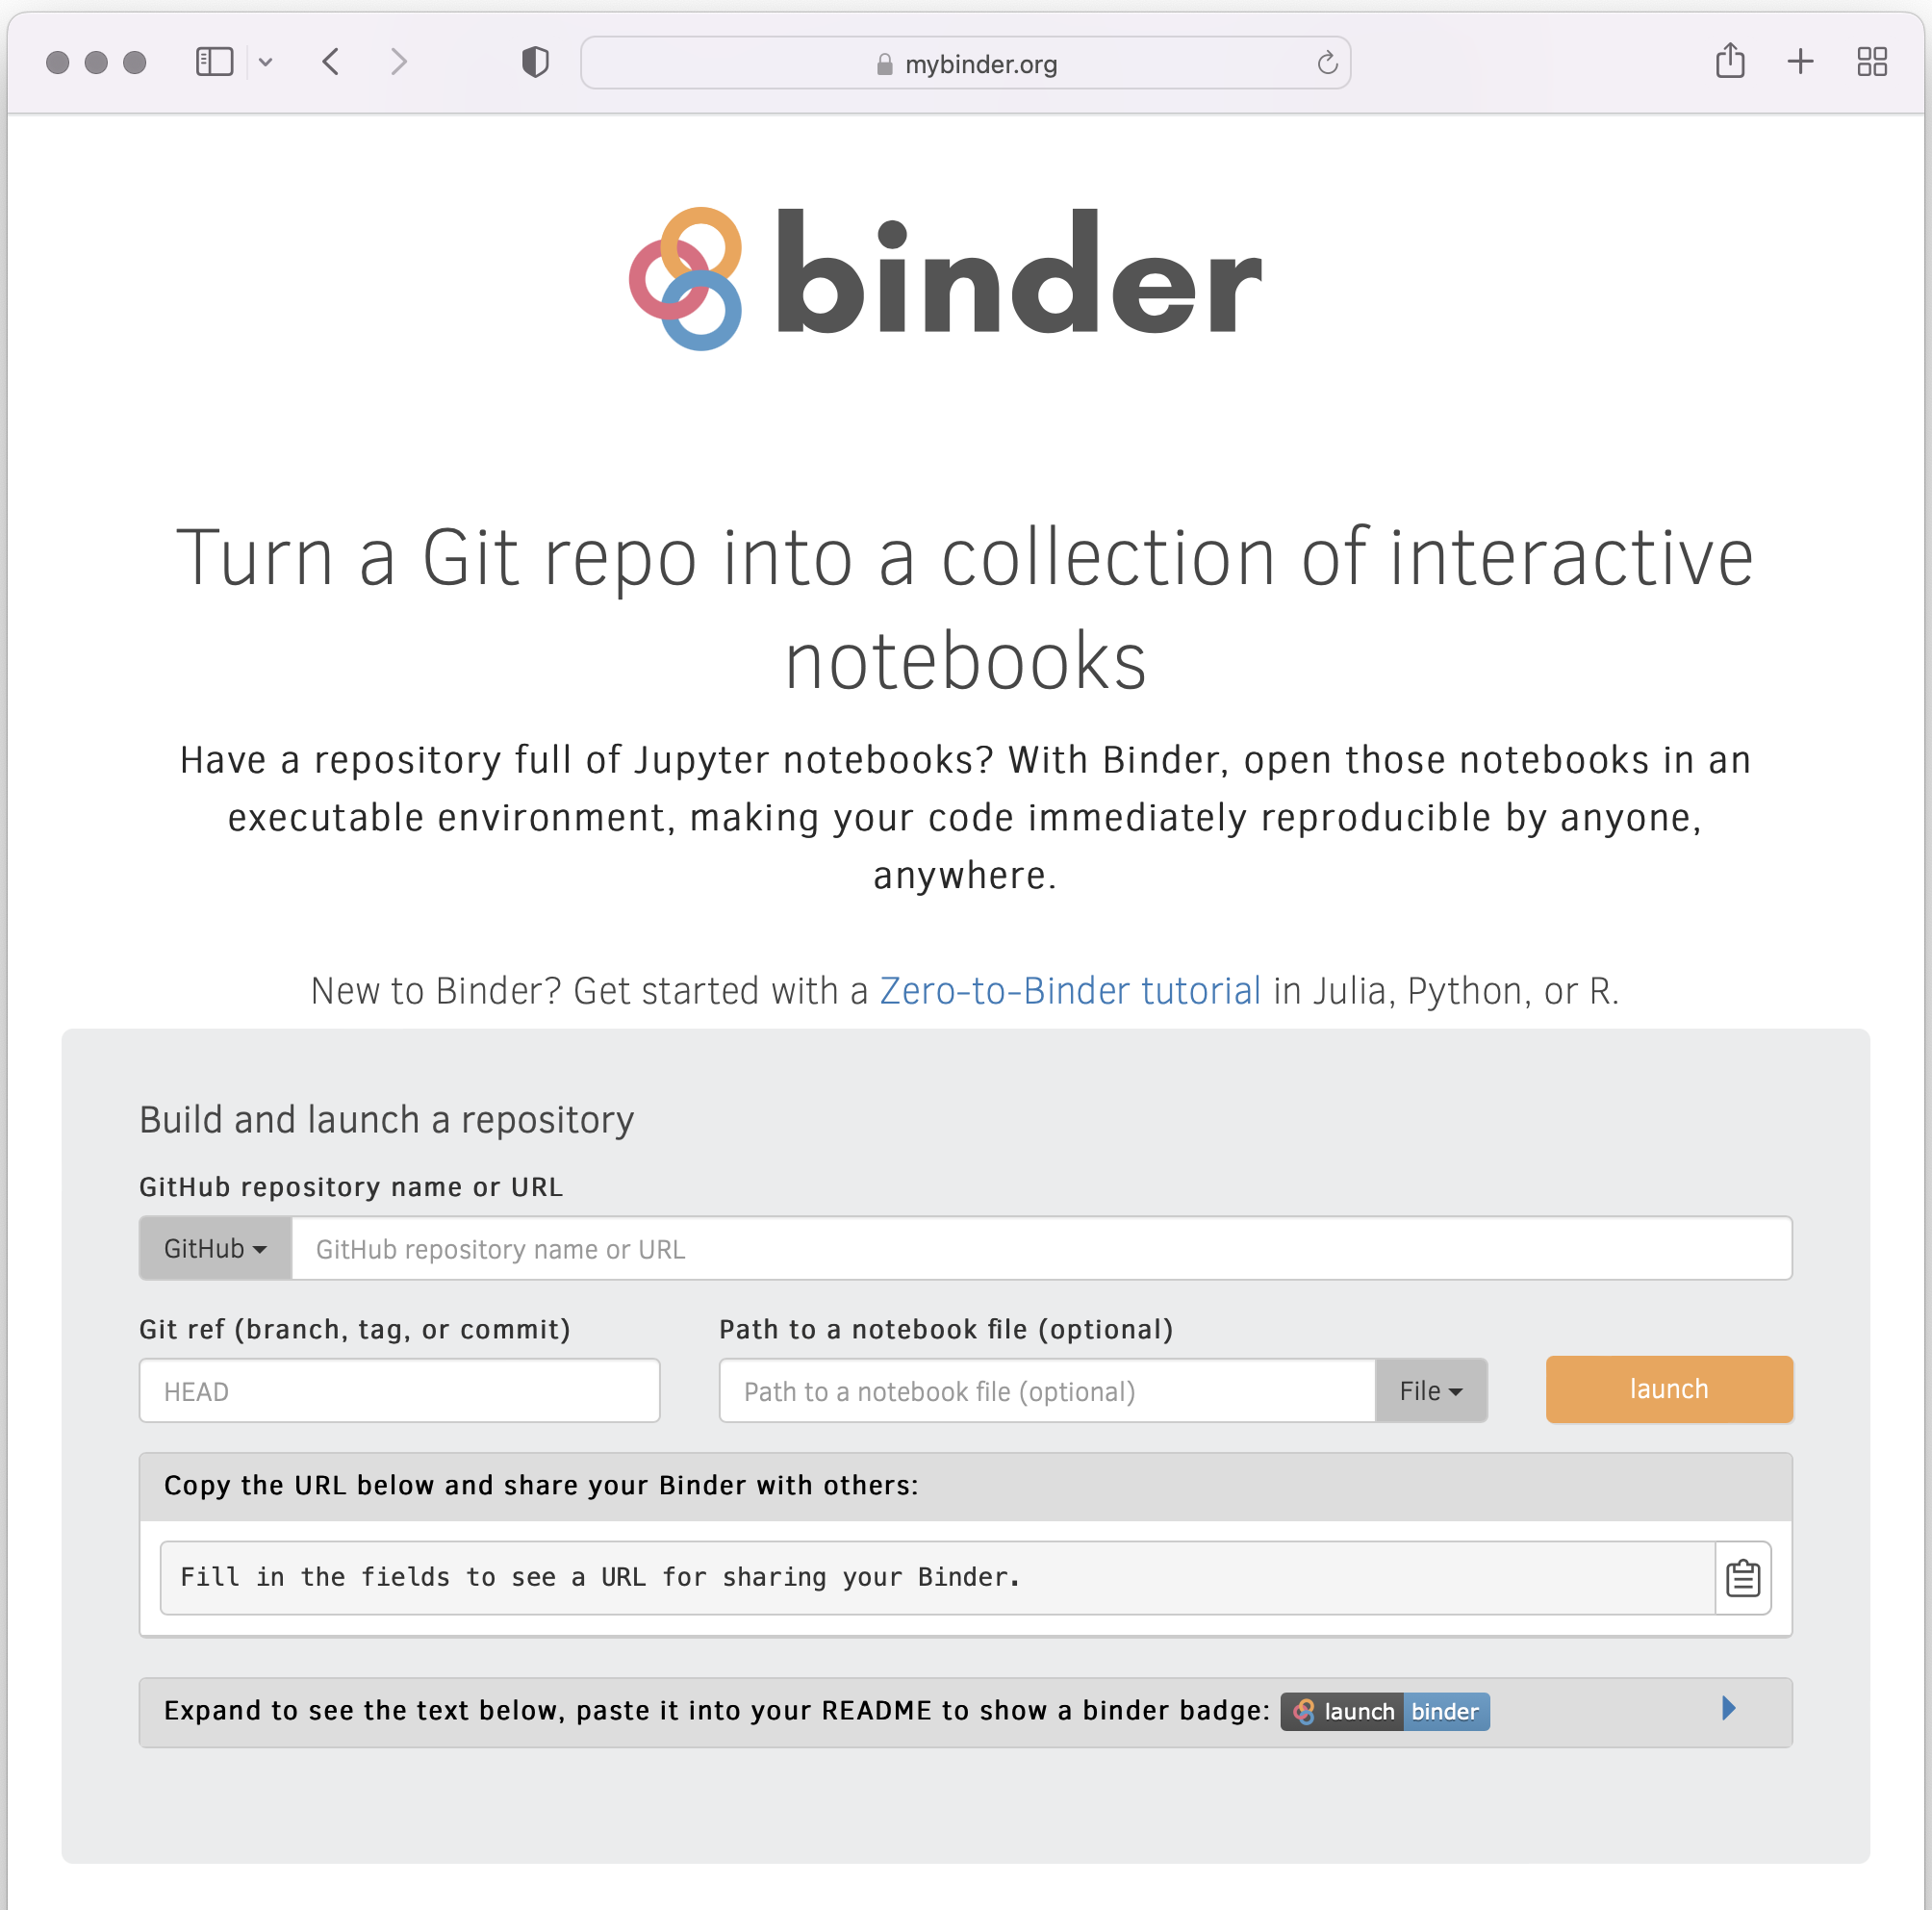
\includegraphics[width=0.7\textwidth]{images/mybinder.png}
    \caption{Home page of the \mybinder{} service.}
    \label{fig:mybinder-homepage}
\end{figure}


\begin{compactitem}
\item The \mybinder{} service is called with a URL that encodes the location of the data
  repository\footnote{For example the
    {\url{https://mybinder.org/v2/gh/fangohr/reproducibility-repository-example/HEAD?labpath=figure1.ipynb}}
    refers to the GitHub repository ``reproducibility-repository-example'' of the
    github user ``fangohr'', asking to open the ``figure1.ipynb'' file.}

  Alternatively, there is form (see Figure~\ref{fig:mybinder-homepage})
  which users can complete with repository details
  to start the build of the corresponding environment, or to obtain the URL to
  re-use that configuration later, or share it with others.
\item From the \mybinder{} entry point, the request is forwarded to one
  \binderhub{} service of one of the organisations in the BinderHub Federation
  that has available compute resources.
\item The \binderhub{} software running at the chosen location, will ask
  \repotodocker{} to create a Docker container in which the notebooks from the repository can be executed.
\item \repotodocker{} searches the repository for specifications of software requirements (see \ref{repo2docker-supported-software-specifications}).
\item \repotodocker{} composes a Dockerfile that contains all the commands
  necessary to install software.
\item \repotodocker{} builds the Docker image based on the Dockerfile.
\item \binderhub{} takes the Docker image and asks Kubernetes to start
  a container based on this image.
\item The notebook server is started in this Docker container.
\item \binderhub{} forwards the user who requested this virtual environment to
  the URL at which the repository (or a particular notebook) can be explored
  from within the Jupyter notebook (which runs in the container).
\end{compactitem}

\subsubsection{The repo2docker software tool.}\label{sec:repo2docker}

\repotodocker{} is a tool to fetch a remote repository and build a software
environment for this repository. Currently, \repotodocker{} can retrieve
repositories from the following services and formats: GitHub, Gist, Git, GitLab,
Zenodo, Hydroshare, Figshare, Dataverse.

For the automatic building of reproducible computational environments,
\repotodocker{} understands commonly used conventions for environment specifications and
community standard tools such as Docker, conda, mamba, and pip. See
Section~\ref{repo2docker-supported-software-specifications} below for a full list of
currently supported software specifications.

\subsubsection{Supported software specification formats}
\label{repo2docker-supported-software-specifications}
The \repotodocker{} tool currently supports the following software specification
formats to build Docker images:
% source:
% https://repo2docker.readthedocs.io/en/latest/config_files.html#config-files
% 9 April 2022
\begin{compactitem}
\item \softwarename{requirements.txt}, \softwarename{setup.py},
  \softwarename{Pipfile}, \softwarename{Pipfile.lock}: to specify Python
  packages and environments
\item \softwarename{Project.toml}, \softwarename{JuliaProject.toml} and (legacy)
  \softwarename{REQUIRE}: to
  specify Julia version and packages
\item \softwarename{install.R}, \softwarename{DESCRIPTION}: to install R
  libraries, or install the repository as R package
\item \softwarename{apt.get}: to install Debian packages. The Docker container
  is currently based on Ubuntu, which uses the Debian package management tool \softwarename{apt}.
\item \softwarename{environment.yml}: to specify conda or mamba packages and
  environments
\item \softwarename{default.nix}: to use the nix package manager for software provision
\item \softwarename{Dockerfile}: providing a Dockerfile enables users to define
  virtually arbitrary environments, for example based on software from the
  repositories of Linux distributions.
\end{compactitem}

\subsubsection{BinderHub}\label{sec:binderhub}
BinderHub is software for hosting a web service built on \repotodocker{} and
JupyterHub where individuals can share reproducible environments for
immediate and free interaction by readers in their browser.


\subsubsection{The \mybinder{} service}\label{sec:mybinder}

\emph{\mybinder{}} is a service run by the \emph{BinderHub
Federation}\footnote{\url{https://mybinder.readthedocs.io/en/latest/about/federation.html}}
of organisations. Collectively, they host a service running the BinderHub software
which can be reached from \url{https://mybinder.org}.

The service is actively used with approximately 200,000 sessions being
requested and delivered by the \mybinder{} service every week in 2021. The number
of sessions is growing from approximately 10,000 per day in November 2018
(beginning of the available records) to about 30,000 per day in 2022. We have
identified 60,000 unique repositories published in the last few years which have
used the \mybinder{} service. The data is available~\cite{mybinder-archive}.

Examples of reproducible repositories that make use of the \mybinder service
include reproducible research repositories
\cite{GitHubRepoExampleAlbert2016,Beg2021}, interactive textbooks
\cite{Fangohr2022,Zeller2022} and citizen science and outreach activities
\cite{ligo-open-science,OSCOVIDA2022}.

This \TheProject{} project will not provide or operate a BinderHub service (such as the global
``\url{https://mybinder.org}'' instance). The improvements achieved, however, will immediately
be made available to all operators of BinderHubs, including \mybinder{}.


% \subsubsection{Binder for reproducibility}\label{sec:binder-for-reproducibility}
% \TOWRITE{}{Hmm -- perhaps we don't need this section, as we explain in the
%   Methodology section what we want to do with Binder?}




%%% Local Variables:
%%% mode: latex
%%% TeX-master: "proposal"
%%% End:
